\documentclass{article}
\usepackage{mathtools}
\usepackage{amsthm, amsfonts, amssymb}
\usepackage{float}
\usepackage{tikz}
\usetikzlibrary{
    arrows.meta,            % Latex and Stealth arrows.
    decorations.markings    % Adding arrows to the middle of line segments.
}

% Define theorem style for default spacing and normal font.
\newtheoremstyle{normal}
    {\topsep}               % Amount of space above the theorem.
    {\topsep}               % Amount of space below the theorem.
    {}                      % Font used for body of theorem.
    {}                      % Measure of space to indent.
    {\bfseries}             % Font of the header of the theorem.
    {}                      % Punctuation between head and body.
    {.5em}                  % Space after theorem head.
    {}

\theoremstyle{normal}
\newtheorem{problem}{Problem}
\newtheorem{definition}{Definition}
\newtheorem{notation}{Notation}

% Italic header environment.
\newtheoremstyle{thmit}{\topsep}{\topsep}{}{}{\itshape}{}{0.5em}{}

% Define environments with italic headers.
\theoremstyle{thmit}
\newtheorem*{solution}{Solution}

\title{Team Taussky\\ Homework 1}
\author{Lizzie Buchanan, Melanie Ferreri, Richard Haburcak,\\
        Matt Jones, Ryan Maguire}
\date{September 2020}

\begin{document}
\maketitle
Olga Taussky-Todd (1906 - 1995 C.E.) was an Austrian mathematician who worked in
algebraic number theory and integral matrices. She produced over 300 research
papers in her lifetime.
\section{Preliminary}
    \begin{definition}
        A graph is a set of vertices with edges connecting pairs of vertices.
    \end{definition}
    \begin{figure}[H]
        \centering
        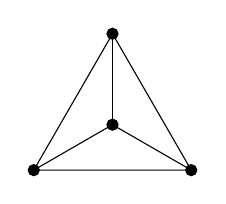
\begin{tikzpicture}
            \coordinate (P1) at (-1, 0.0);
            \coordinate (P2) at (1, 0.0);
            \coordinate (P3) at (0, 1.73205);
            \coordinate (P4) at (0, 0.57735);

            \draw (P1) to (P2) to (P3) to cycle;
            \draw (P1) to (P4);
            \draw (P2) to (P4);
            \draw (P3) to (P4);

            \draw[fill=black] (P1) circle (2pt);
            \draw[fill=black] (P2) circle (2pt);
            \draw[fill=black] (P3) circle (2pt);
            \draw[fill=black] (P4) circle (2pt);
        \end{tikzpicture}
        \caption{A Graph}
        \label{fig:Graph_Example}
    \end{figure}
    \begin{definition}
        A connected graph is one where you can walk between any two
        vertices along the edges of G.
    \end{definition}
    \begin{definition}
        A tree is a graph with no cycles.
    \end{definition}
    \par
    \begin{minipage}[b]{0.47\textwidth}
        \centering
        \begin{figure}[H]
        \centering
            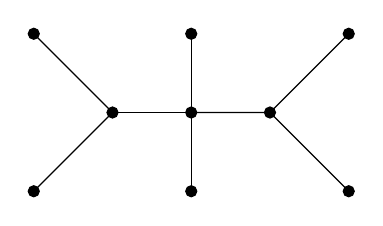
\begin{tikzpicture}
                \coordinate (P0) at (-2.0,  1.0);
                \coordinate (P1) at (-2.0, -1.0);
                \coordinate (P2) at (-1.0,  0.0);
                \coordinate (P3) at ( 0.0,  0.0);
                \coordinate (P4) at ( 0.0,  1.0);
                \coordinate (P5) at ( 0.0, -1.0);
                \coordinate (P6) at ( 1.0,  0.0);
                \coordinate (P7) at ( 2.0,  1.0);
                \coordinate (P8) at ( 2.0, -1.0);

                \draw (P0) to (P2) to (P1);
                \draw (P2) to (P3);
                \draw (P4) to (P3) to (P5);
                \draw (P3) to (P6) to (P7);
                \draw (P6) to (P8);

                \draw[fill=black] (P0) circle (2pt);
                \draw[fill=black] (P1) circle (2pt);
                \draw[fill=black] (P2) circle (2pt);
                \draw[fill=black] (P3) circle (2pt);
                \draw[fill=black] (P4) circle (2pt);
                \draw[fill=black] (P5) circle (2pt);
                \draw[fill=black] (P6) circle (2pt);
                \draw[fill=black] (P7) circle (2pt);
                \draw[fill=black] (P8) circle (2pt);
            \end{tikzpicture}
            \caption{A Tree}
            \label{fig:Tree_Example}
        \end{figure}
    \end{minipage}
    \hfill
    \begin{minipage}[b]{0.47\textwidth}
        \centering
        \begin{figure}[H]
            \centering
            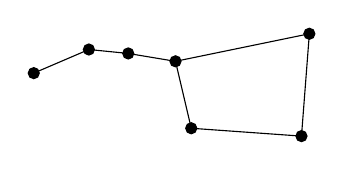
\begin{tikzpicture}
                \coordinate (P0) at (-2.0,  0.0);
                \coordinate (P1) at (-1.3,  0.3);
                \coordinate (P2) at (-0.8,  0.25);
                \coordinate (P3) at (-0.2,  0.15);
                \coordinate (P4) at ( 1.5,  0.5);
                \coordinate (P5) at ( 1.4, -0.8);
                \coordinate (P6) at ( 0.0, -0.7);

                \draw (P0) to (P1) to (P2) to (P3) to (P4)
                           to (P5) to (P6) to (P3);

                \draw[fill=black] (P0) circle (2pt);
                \draw[fill=black] (P1) circle (2pt);
                \draw[fill=black] (P2) circle (2pt);
                \draw[fill=black] (P3) circle (2pt);
                \draw[fill=black] (P4) circle (2pt);
                \draw[fill=black] (P5) circle (2pt);
                \draw[fill=black] (P6) circle (2pt);
            \end{tikzpicture}
            \caption{Not a Tree}
            \label{fig:ExampleNotATree}
        \end{figure}
    \end{minipage}
    \begin{notation}
        If $G$ is a graph and $e$ is an edge in $G$, we write $G\setminus{e}$ to denote
        the graph obtained by removing $e$.
    \end{notation}
    \begin{figure}[H]
        \centering
        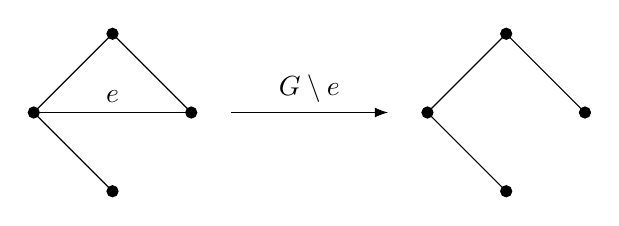
\begin{tikzpicture}[>=Latex]
            \coordinate (P1) at ( 0, -1);
            \coordinate (P2) at (-1,  0);
            \coordinate (P3) at ( 1,  0);
            \coordinate (P4) at ( 0,  1);

            \coordinate (Q1) at (5, -1);
            \coordinate (Q2) at (4,  0);
            \coordinate (Q3) at (6,  0);
            \coordinate (Q4) at (5,  1);
        
            \draw (P1) to (P2) to (P4) to (P3);
            \draw (P3) to node[above] {$e$} (P2);
        
            \draw[fill=black] (P1) circle (2pt);
            \draw[fill=black] (P2) circle (2pt);
            \draw[fill=black] (P3) circle (2pt);
            \draw[fill=black] (P4) circle (2pt);

            \draw[->, shorten <=0.5cm, shorten >=0.5cm]
                (P3) to node[above] {$G\setminus{e}$} (Q2);

            \draw (Q1) to (Q2) to (Q4) to (Q3);

            \draw[fill=black] (Q1) circle (2pt);
            \draw[fill=black] (Q2) circle (2pt);
            \draw[fill=black] (Q3) circle (2pt);
            \draw[fill=black] (Q4) circle (2pt);
        \end{tikzpicture}
        \caption{Removal of an Edge}
        \label{fig:EdgeRemoval}
    \end{figure}
    \begin{notation}
        If $G$ is a graph and $e$ is an edge in $G$, we write $G/e$ to
        denote the graph obtained from $G$ by contracting $e$.
    \end{notation}
    \begin{figure}[H]
        \centering
        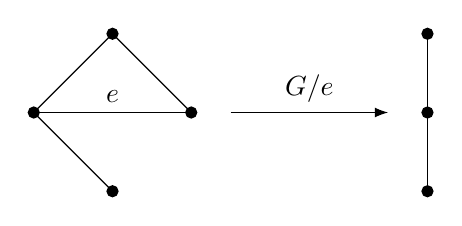
\begin{tikzpicture}[>=Latex]
            \coordinate (P1) at ( 0, -1);
            \coordinate (P2) at (-1,  0);
            \coordinate (P3) at ( 1,  0);
            \coordinate (P4) at ( 0,  1);

            \coordinate (Q1) at (4, -1);
            \coordinate (Q2) at (4,  0);
            \coordinate (Q3) at (4,  1);
        
            \draw (P1) to (P2) to (P4) to (P3);
            \draw (P3) to node[above] {$e$} (P2);
        
            \draw[fill=black] (P1) circle (2pt);
            \draw[fill=black] (P2) circle (2pt);
            \draw[fill=black] (P3) circle (2pt);
            \draw[fill=black] (P4) circle (2pt);

            \draw[->, shorten <=0.5cm, shorten >=0.5cm]
                (P3) to node[above] {$G/{e}$} (Q2);

            \draw (Q1) to (Q2) to (Q3);

            \draw[fill=black] (Q1) circle (2pt);
            \draw[fill=black] (Q2) circle (2pt);
            \draw[fill=black] (Q3) circle (2pt);
        \end{tikzpicture}
        \caption{Contracting of an Edge}
        \label{fig:EdgeContraction}
    \end{figure}
    \begin{definition}
        A $\lambda$ coloring of a graph $G$ is an assignment of colors taken
        from $\{C_{1},\dots,C_{\lambda}\}$ so that every pair of adjacent
        vertices have different colors.
    \end{definition}
    \begin{figure}[H]
        \centering
        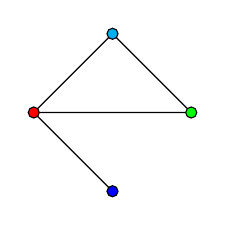
\begin{tikzpicture}
            \coordinate (P1) at (0, -1);
            \coordinate (P2) at (-1, 0);
            \coordinate (P3) at (1, 0);
            \coordinate (P4) at (0, 1);
        
            \draw (P1) to (P2) to (P4) to (P3) to (P2);
        
            \draw[fill=blue] (P1) circle (2pt);
            \draw[fill=red] (P2) circle (2pt);
            \draw[fill=green] (P3) circle (2pt);
            \draw[fill=cyan] (P4) circle (2pt);
        \end{tikzpicture}
        \caption{A 4-coloring of $G$}
        \label{fig:LambdaColoring}
    \end{figure}
    \begin{notation}
        If $G$ is a graph, then $\chi_{G}(\lambda)$ denotes to the total number of
        $\lambda$ colorings of $G$.
    \end{notation}
    \begin{definition}
        An acyclic orientation of a graph $G$ is an assignment of directions to each
        edge of $G$ so that there are no directed cycles.
    \end{definition}
    \begin{notation}
        If $G$ is a graph, then we write $a_{G}$ to denote the number of acyclic
        orientations of $G$.
    \end{notation}
\section{Problems}
    \begin{figure}[H]
        \centering
        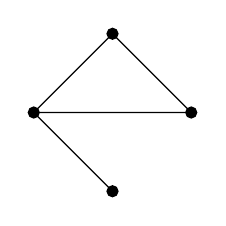
\begin{tikzpicture}
            \coordinate (P1) at (0, -1);
            \coordinate (P2) at (-1, 0);
            \coordinate (P3) at (1, 0);
            \coordinate (P4) at (0, 1);
        
            \draw (P1) to (P2) to (P4) to (P3) to (P2);
        
            \draw[fill=black] (P1) circle (2pt);
            \draw[fill=black] (P2) circle (2pt);
            \draw[fill=black] (P3) circle (2pt);
            \draw[fill=black] (P4) circle (2pt);
        \end{tikzpicture}
        \caption{The Graph Being Considered}
        \label{fig:TheGraph}
    \end{figure}
    \begin{problem}
        Determine $\chi_G(\lambda)$ and $a_G$ for $G$ as given.
    \end{problem}
    \begin{solution}
        To compute $\chi_{G}(\lambda)$ we first consider a few cases of $\lambda$. There
        are no 1-colorings since $G$ is connected and there are no 2-colorings since
        the graph contains a closed triangle and hence a minimum of 3 colors is needed.
        If $\lambda\geq{3}$ then we can do the following. Label the bottom vertex any
        color. There are $\lambda$ ways, and there is only one vertex adjacent to the
        bottom leaving $\lambda-1$ ways to color this one. The other two vertices are
        not adjacent to the bottom, so this frees up one of the colors. Hence there are
        $\lambda-1$ colors available for one of them and $\lambda-2$ for the other. This
        gives us:
        \begin{equation}
            \chi_{G}(\lambda)=\lambda(\lambda-1)(\lambda-1)(\lambda-2)
        \end{equation}
        An example of a 3-coloring of $G$ is shown in Fig.~\ref{fig:ThreeColoring}.
        Note the top and bottom vertices are allowed to have the same color since they
        are not adjacent.
            \begin{figure}[H]
                \centering
                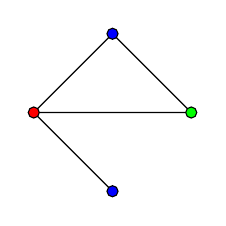
\begin{tikzpicture}
                    \coordinate (P1) at (0, -1);
                    \coordinate (P2) at (-1, 0);
                    \coordinate (P3) at (1, 0);
                    \coordinate (P4) at (0, 1);
                
                    \draw (P1) to (P2) to (P4) to (P3) to (P2);
                
                    \draw[fill=blue] (P1) circle (2pt);
                    \draw[fill=red] (P2) circle (2pt);
                    \draw[fill=green] (P3) circle (2pt);
                    \draw[fill=blue] (P4) circle (2pt);
                \end{tikzpicture}
                \caption{A 3-coloring of $G$}
                \label{fig:ThreeColoring}
            \end{figure}
        We can compute $a_{G}$ by counting the total number of possible combinations of
        directed arrows, and then subtract off the cyclic ones. Since there are 4 edges
        with 2 possible directions each, there are $2^{4}=16$ possible directed graphs on
        $G$. To have a cycle we would need the triangular part to either be clockwise or
        counterclockwise, the direction of the bottom-most edge is irrelevant. So, 2
        cycles per direction of the bottom-most edge, giving us 4 non-acyclic graphs.
        Hence, $a_{G}=16-4=12$. The non-acyclic graphs are shown in
        Fig.~\ref{fig:NonAcyclicGraphs}.
    \end{solution}
    \begin{figure}[H]
        \centering
        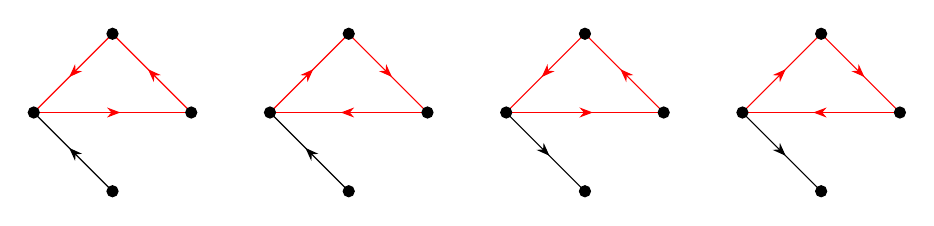
\begin{tikzpicture}[%
            ->-/.style={%
                    decoration={%
                        markings,
                        mark=at position .55 with \arrow{Stealth}
                    },
                    postaction={decorate}
                }
            ]
            \newcommand*{\defcoords}{%
                \coordinate (P1) at (0, -1);
                \coordinate (P2) at (-1, 0);
                \coordinate (P3) at (1, 0);
                \coordinate (P4) at (0, 1);
            }

            \defcoords;
            \draw[->-] (P1) to (P2);
            \draw[red, ->-] (P2) to (P3);
            \draw[red, ->-] (P3) to (P4);
            \draw[red, ->-] (P4) to (P2);
            
            \draw[fill=black] (P1) circle (2pt);
            \draw[fill=black] (P2) circle (2pt);
            \draw[fill=black] (P3) circle (2pt);
            \draw[fill=black] (P4) circle (2pt);

            \begin{scope}[xshift=3cm]
                \defcoords;
                \draw[->-] (P1) to (P2);
                \draw[red, ->-] (P3) to (P2);
                \draw[red, ->-] (P4) to (P3);
                \draw[red, ->-] (P2) to (P4);

                \draw[fill=black] (P1) circle (2pt);
                \draw[fill=black] (P2) circle (2pt);
                \draw[fill=black] (P3) circle (2pt);
                \draw[fill=black] (P4) circle (2pt);
            \end{scope}

            \begin{scope}[xshift=6cm]
            \defcoords;
                \draw[->-] (P2) to (P1);
                \draw[red, ->-] (P2) to (P3);
                \draw[red, ->-] (P3) to (P4);
                \draw[red, ->-] (P4) to (P2);
                
                \draw[fill=black] (P1) circle (2pt);
                \draw[fill=black] (P2) circle (2pt);
                \draw[fill=black] (P3) circle (2pt);
                \draw[fill=black] (P4) circle (2pt);
            \end{scope}

            \begin{scope}[xshift=9cm]
                \defcoords;
                \draw[->-] (P2) to (P1);
                \draw[red, ->-] (P3) to (P2);
                \draw[red, ->-] (P4) to (P3);
                \draw[red, ->-] (P2) to (P4);

                \draw[fill=black] (P1) circle (2pt);
                \draw[fill=black] (P2) circle (2pt);
                \draw[fill=black] (P3) circle (2pt);
                \draw[fill=black] (P4) circle (2pt);
            \end{scope}
            \let\defcoords\undefined
        \end{tikzpicture}
        \caption{The non-Acyclic Orientations of $G$}
        \label{fig:NonAcyclicGraphs}
    \end{figure}
    \begin{problem}
        Let $T$ be a tree, find $\chi_G(\lambda)$ and $a_G$ for the tree.
    \end{problem}
    \begin{solution}
        For any root of the tree, we can color with $\lambda$ colors. Then for any
        vertex distance $k$ away from the root, it is connected by a unique edge to the
        subgraph of vertices distance $k-1$ away, hence can be colored by $\lambda -1$
        colors. Thus $\chi_G(\lambda)=\lambda(\lambda-1)^{n-1}$. For $a_G$, we can simply
        orient any edge in any way as $G$ has no cycles. Thus $a_G=2^{n-1}$, as there are
        $n-1$ edges in a tree.
    \end{solution}
    \begin{problem}
        Let $G$ be a graph, and $e$ and edge. Show that
        $\chi_G=\chi_{G\setminus{e}}-\chi_{G/e}$
    \end{problem}
    \begin{solution}
        This follows from counting the colorings of $G\setminus{e}$. For any coloring of $G\setminus{e}$,
        we can get a coloring of $G$ if the ends of the removed edge are different colors.
        However, they may have the same color, which corresponds exactly to a coloring
        of $G/e$.
    \end{solution}
    \begin{problem}
        Deduce the following:
            \begin{enumerate}
                \item $\chi_G$ is a monic  polynomial of degree $n=\vert V(G)\vert$
                    \begin{solution}
                        By the recurrence relation, it suffices to show this for trees, as eventually we
                        get down to a tree by deleting or contracting edges. This was shown above. (We also note that we obtain a tree of $n$ vertices only if we perform repeated deletions. So only one tree contributes to our leading term $\lambda^n$, and as shown above the polynomial for trees is monic. So our $\chi_G$ is monic as well.)
                    \end{solution}
                \item The coefficients of $\chi_G$ are integers and alternate sign.
                    \begin{solution}
                        By the recurrence relation, this follows from the following:
                        \begin{subequations}
                            \begin{align}
                                \chi_G(\lambda)&= \lambda^n +\cdots\\
                                    &=\chi_{G\setminus{e}}(\lambda)-\chi_{G/e}(\lambda)\\
                                    &=\left(\lambda^n+\cdots\right)-\left(
                                        \lambda^{n-1}+\cdots\right)    
                            \end{align}
                        \end{subequations}
                        whereby it follows from induction on the number of vertices.
                    \end{solution}
                \item
                    $\lambda^c$ is a factor of $\chi_G(\lambda)$ where
                    $c=\vert \text{connected components of } G\vert$.
                    \begin{solution}
                        This follows as colorings of different components are independent. Thus
                        $\chi_{G\sqcup H} = \chi_G \cdot \chi_H$ for two graphs $G,H$. (For a graph $G$, we note that $\chi_G(0)=0$ as there are no ways to color a graph with zero colors. Hence $\lambda\vert \chi_G (\lambda)$.)
                    \end{solution}
            \end{enumerate}
    \end{problem}
    \begin{problem}
        Show that $a_G = a_{G\setminus{e}} + a_{G/e}$
    \end{problem}
    \begin{solution}
        Given an acyclic orientation $\mathcal{O}$ of $G\setminus{e}$, we can potentially get 2 acyclic
        orientations $\mathcal{O}_1$, $\mathcal{O}_2$ of $G$ by adding in the edge $e$ in either
        orientation. We claim that either exactly 1 of $\mathcal{O}_1$ or $\mathcal{O}_2$ works, or
        both of them work in which case we have an acyclic orientation of $G/e$. The recurrence then
        follows.
        \par
        If only 1 of $\mathcal{O}_1$, $\mathcal{O}_2$ give an acyclic orientation of $G$, then in $G/e$, the
        contracted orientations $\widetilde{\mathcal{O}_1}$ and $\widetilde{\mathcal{O}_2}$ cannot be an acyclic
        orientation of $G/e$ as we needed the edge $e$ placed in a certain position to prevent a cycle. Thus
        with the edge $e$ contracted, it cannot prevent a cycle in $G/e$.
        \par
        We claim that at least one of $\mathcal{O}_1$ or $\mathcal{O}_2$ do in fact give an acyclic
        orientation of $G$. If this were not the case, then any orientation of $e$ creates a cycle in $G$.
        But if $e$ is contained in an oriented cycle, then reversing that orientation either makes a new
        oriented cycle or gives an acyclic orientation of $G$. Now if reversing the orientation of $e$ were
        to give a new cycle, then the two cycles that $e$ was contained in for both orientations
        $\mathcal{O}_1$, $\mathcal{O}_2$ of $G$ would create a cycle in $G\setminus{e}$, thus
        $\mathcal{O}$ was not acyclic. Therefore at least one of $\mathcal{O}_1$ or $\mathcal{O}_2$ do in
        fact give an acyclic orientation of $G$.
        \par
        Thus given an acyclic orientation of $G\setminus{e}$, we get either 1 acyclic orientation of $G$ or
        2 where we also get one for $G/e$. The recurrence now follows.
    \end{solution}
    \begin{problem}
        Deduce that $a_G = (-1)^n \chi_G(-1)$
    \end{problem}
    \begin{solution}
        This follows at once from the recurrence, as $\vert V(G\setminus{e})\vert = \vert V(G)\vert$, and
        $\vert V(G/e)\vert = \vert V(G)\vert-1$. By induction on the number of edges: we can do a
        base-case, say a forest with no edges (in which case both sides are 0). Then we use "strong"
        induction on the RHS of $a_G = a_{G\setminus{e}} + a_{G/e}$, as $G\setminus{e}$ and $G/e$ have
        fewer edges than $G$ the result holds for them. We then compute:
        \begin{subequations}
            \begin{align}
                a_G&=a_{G\setminus{e}}+a_{G/e}\\
                    &=(-1)^{\vert V(G\setminus{e})\vert}
                        \chi_{G\setminus{e}}(-1)+(-1)^{\vert V(G)\vert -1}\chi_{G/e}(-1)\\
                    &=(-1)^{n}\chi_{G\setminus{e}}(-1) +(-1) (-1) (-1)^{n-1} \chi_{G/e}(-1)\\
                    &=(-1)^{n}\left(\chi_{G\setminus{e}}(-1) - \chi_{G/e}(-1) \right)\\
                    &=(-1)^{n}\chi_{G}(-1)
            \end{align}
        \end{subequations}
    \end{solution}
    \begin{problem}
        Compute $\operatorname{dim}(\Delta_r(G))$ for $G$ given, and $r=-1,0,1$.
    \end{problem}
    \begin{solution}
    This is a simple matter of counting the number of possible ordered partitions that contain an edge.
    \begin{itemize}
        \item[$r=-1$]
            There is only one partition into one set, $\{1,2,3,4\}$. Since there is only one
            partition, it can only be ordered one way, and therefore there is one basis vector
            and one dimension.
        \item[$r=0$]
            There are six partitions into two sets:
            \begin{equation}
                \begin{split}
                    &\big(\{1,2,3\},\{4\}\big),\;\big(\{1,2\},\{3,4\}\big),\;
                        \big(\{1,2,4\},\{3\}\big),\\
                    &\big(\{1\},\{2,3,4\}\big),\;\big(\{2\},\{1,3,4\}\big),\;
                        \big(\{1,4\},\{2,3\}\big)
                \end{split}
            \end{equation}
            Each partition has two possible orderings, so the dimension is $6*2=12$. 
        \item[$r=1$]
            There are three partitions:
            \begin{equation}
                \big(\{1,2\},\{3\},\{4\}\big),\;
                \big(\{1\},\{2,3\},\{4\}\big),\;
                \big(\{1\},\{2\},\{3,4\}\big)
            \end{equation}
            Each partition now has 6 orderings, and the dimension is 18.
    \end{itemize}
    \end{solution}
    \begin{problem}
        Show $d_r \circ d_{r+1} =0$
    \end{problem}
    \begin{solution}
        $d_r \circ d_{r+1} (B_1, \dots, B_{r+2})$ is the sum of a collection of partitions in which there
        are two unions, ie $\pm(B_1, \dots, B_i \cup B_{i+1}, \dots B_j \cup B_{j+1}, \dots B_{r+2})$.
        However, each term appears twice, once with $B_i, B_{i+1}$ being unioned first, and once with
        $\dots B_j \cup B_{j+1}$ first. But because of the $(-1)^{i-1}$ in the definition of $d_r$, they
        will have oppposite signs. Therefore, all similar terms will cancel out and $d_r \circ d_{r+1} =0$.
    \end{solution}
\end{document}
